In order to have an upper bound for the LU decomposition with partial pivoting, we also implemented an LU decomposition with static pivoting. It is similar to a partial pivoting but without swapping operation. It may be considered as a Cholesky's algorithm applied to the two sides of the matrix.

\dague includes already an implementation of LU decomposition with incremental pivoting. Thus, we compare them with the performances obtained of partial pivoting.

To complete the experiences, we also compare results with Scalapack performances.

\section*{Exploiting hierarchical platform with PTG}
For this experience, we used \dague as PTG runner. The architecture used is and hierarchical platform. It consists of 128 cores - Intel(R) Xeon(R) E5220 - distributed over 16 nodes and interconnected with an Infini Band. Each core runs with a frequency of 2.27GHz. 

We implemented Task flow \ref{fig:hybrid_task_flow} for panel factorization and Task flow \ref{fig:update_task_flow} for swapping operations in update. The softwares used are Linux as operating system, \dague as runtime system and the Intel Mkl library version 11.1 for Blas routines. We used the sequential version of BLAS in \dague but the Scalapack tests ran with parallel BLAS routines (PBLAS).

\begin{figure}
\centering
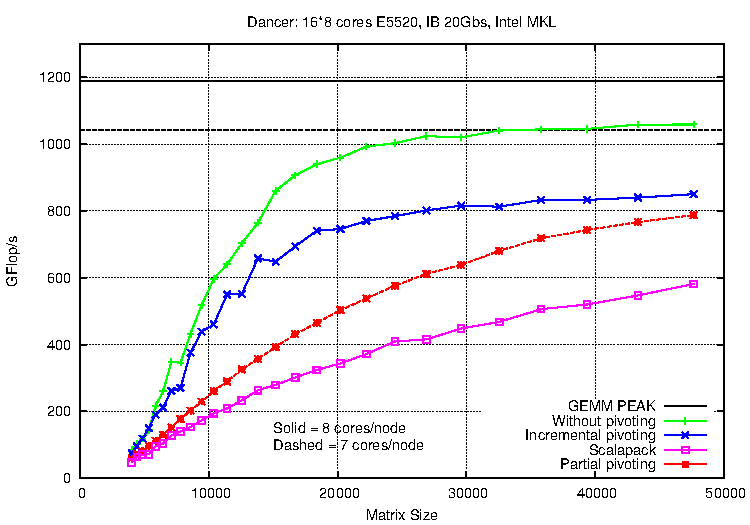
\includegraphics[width=0.8\textwidth]{figures/gepp.pdf}
\caption{Performance of LU decomposition with PTG\label{fig:pp}} 
\end{figure}

The partial pivoting implemented was ran with only 7 cores by node for computation. The eighth core was completely dedicated to the communication. In fact, experiments show that is more efficient to allow one core to manage the huge number of small communications on the panel. In the figure \ref{fig:pp}, it is showed two \emph{gemm} peak, one using 8 core and the other only 7. The results obtained are satisfying. In fact, the red curve - which is our implementation of LU decomposition over \dague - reaches 75\% of the \emph{gemm} peak. Moreover, the performance of our LU decomposition is far better than Scalpack which is one of the most used mathematical library by the scientist community. The curves of the LU decomposition with incremental pivoting and without pivoting have better performances because their algorithms have less synchronisations, but their numerical values of their results are not accurate.

%\section{Exploiting heterogeneous platform with sequential task flow}


%The distributed tests was applied on a machine of 16 nodes of 8 cores each, using an Infini Band network and the Intel MKL library.
%The first experiment applied was to take the static pivoting and plug on it the update engine implemented. Because all communications are done in every case, this test give the cost of the execution of the update engine. The result is showen in the figure \ref{fig:update}. The first remark is that the static pivoting is quickly approaching the gemm peak computer. This can be explained by the fact that all the getrf and trsm operations are recovered by gemm. The second curve is just a little below the first one. Thus, the update engine has a very small impact on the performances despite of its entire execution.  This is a very good result because first the update engine is generic and second its cost is very low.
%\begin{figure}
%\centering
%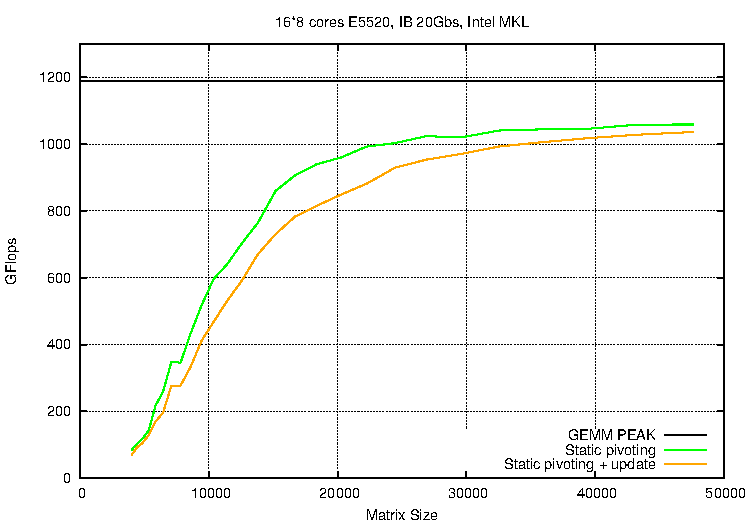
\includegraphics[width=0.8\textwidth]{figures/dgetrf_update_problem.pdf}
%\caption{Impact of the update engine on the performances\label{fig:update}} 
%\end{figure}
%The second experiment applied was the testing of the LU decomposition with partial pivoting implemented. It was compared to the incremental pivoting and the Scalapack implementation. At the moment, the partial pivoting implemented was runned with only 7 cores by node for computation. The eighth core was completly dedicated to the communication. This was necesary to manage the high number of small communications on the panel. In the figure \ref{fig:pp}, it is showed two gemm peak, one using 8 core and the other only 7.
%\begin{figure}
%\centering
%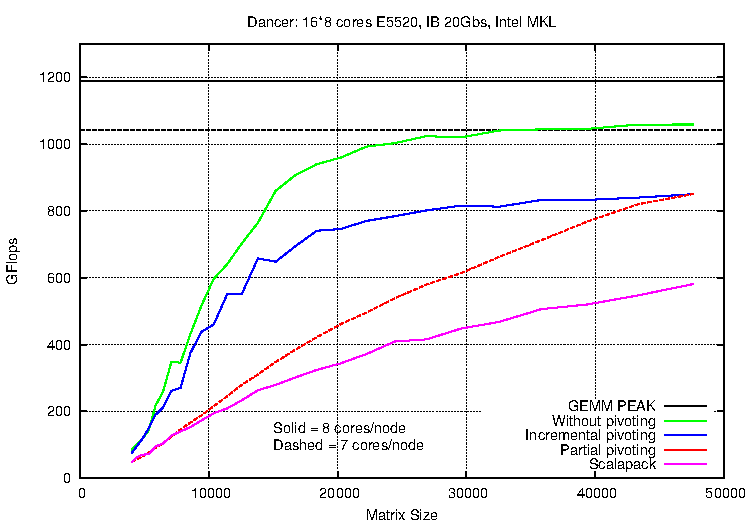
\includegraphics[width=0.8\textwidth]{figures/partial_pivoting_problem.pdf}
%\caption{Impact of the update engine on the performances\label{fig:pp}} 
%\end{figure}
